\chapter{Implementation}
The application is implemented as a `mini-app' of the \textit{TrustChain Superapp}~\citep{mattskala2020}. This follows the concept of super apps~\citep{kpmg2019superapps}. The app is published on the Android Play Store\footnote{\url{https://play.google.com/store/apps/details?id=nl.tudelft.trustchain}} and runs on Android 5.1 and above. Its code is publicly available\footnote{\url{https://github.com/Tim-W/trustchain-superapp}}. As programming language Kotlin is selected, as it is the preferred language for Android development\footnote{\url{https://android-developers.googleblog.com/2019/05/google-io-2019-empowering-developers-to-build-experiences-on-Android-Play.html}}. Moreover the underlying technology stack is also written in Kotlin, so this allows for neat integration. This section describes the implementation choices, usage of external libraries and presents the user interface of MusicDAO. The main interfaces of the app can be seen below (figs. \ref{fig:screenshot-home}, \ref{fig:screenshot-playlist} and \ref{fig:tip-artist}). An overview of the structure of the code can be seen in the package diagram in fig. \ref{fig:package-diagram}.

\section{Features overview}
We implemented a peer-to-peer system to share, discover and listen to music, and to give payments to artists. 100\% of money goes to artists. The system requires no servers, middlemen or third parties to run, and is resilient: it can not be taken down by any government or institution. Our Android app contains the following features:
\begin{itemize}
    \item Defining album/single/EP releases using metadata, and sharing those with peers; Sharing of your audio tracks with peers; Immutable storage of music metadata and cryptographic identification of artists.
    \item Streaming music over BitTorrent; Prioritization algorithm to minimize streaming latency; Caching audio files and metadata.
    \item Browsing playlists; Local and remote keyword search for music.
    \item Mobile bitcoin wallet implementation; Peer-to-peer donations to artists using Bitcoin.
\end{itemize}
The following planned features were not implemented:
\begin{itemize}
    \item Artist Income Division Algorithm.
    \item Content sorting algorithm based on swarm health.
\end{itemize}
Apart from the Android SDK and the TrustChain Superapp, the main libraries that are used are shown in \ref{tab:library-usage}. In the following sections we explain the details of implementing the aforementioned features in a top-down overview, starting with the interfaces.

\begin{table}[]
\begin{tabular}{|l|l|l|}
\hline
Name                  & Version & Usage                          \\ \hline
JLibtorrent           & 1.2.10  & Peer-to-peer file distribution \\ \hline
TorrentStream-Android & 2.7.0   & Video streaming library        \\ \hline
ExoPlayer             & 2.10.5  & Android multimedia player      \\ \hline
BitcoinJ              & 0.15.7  & Java bitcoin interface         \\ \hline
XChange               & 5.0.1   & Crypto/USD price conversion    \\ \hline
\end{tabular}
\caption{Notable libraries used}
\label{tab:library-usage}
\end{table}

\begin{figure}[]
    \minipage{0.3\textwidth}
        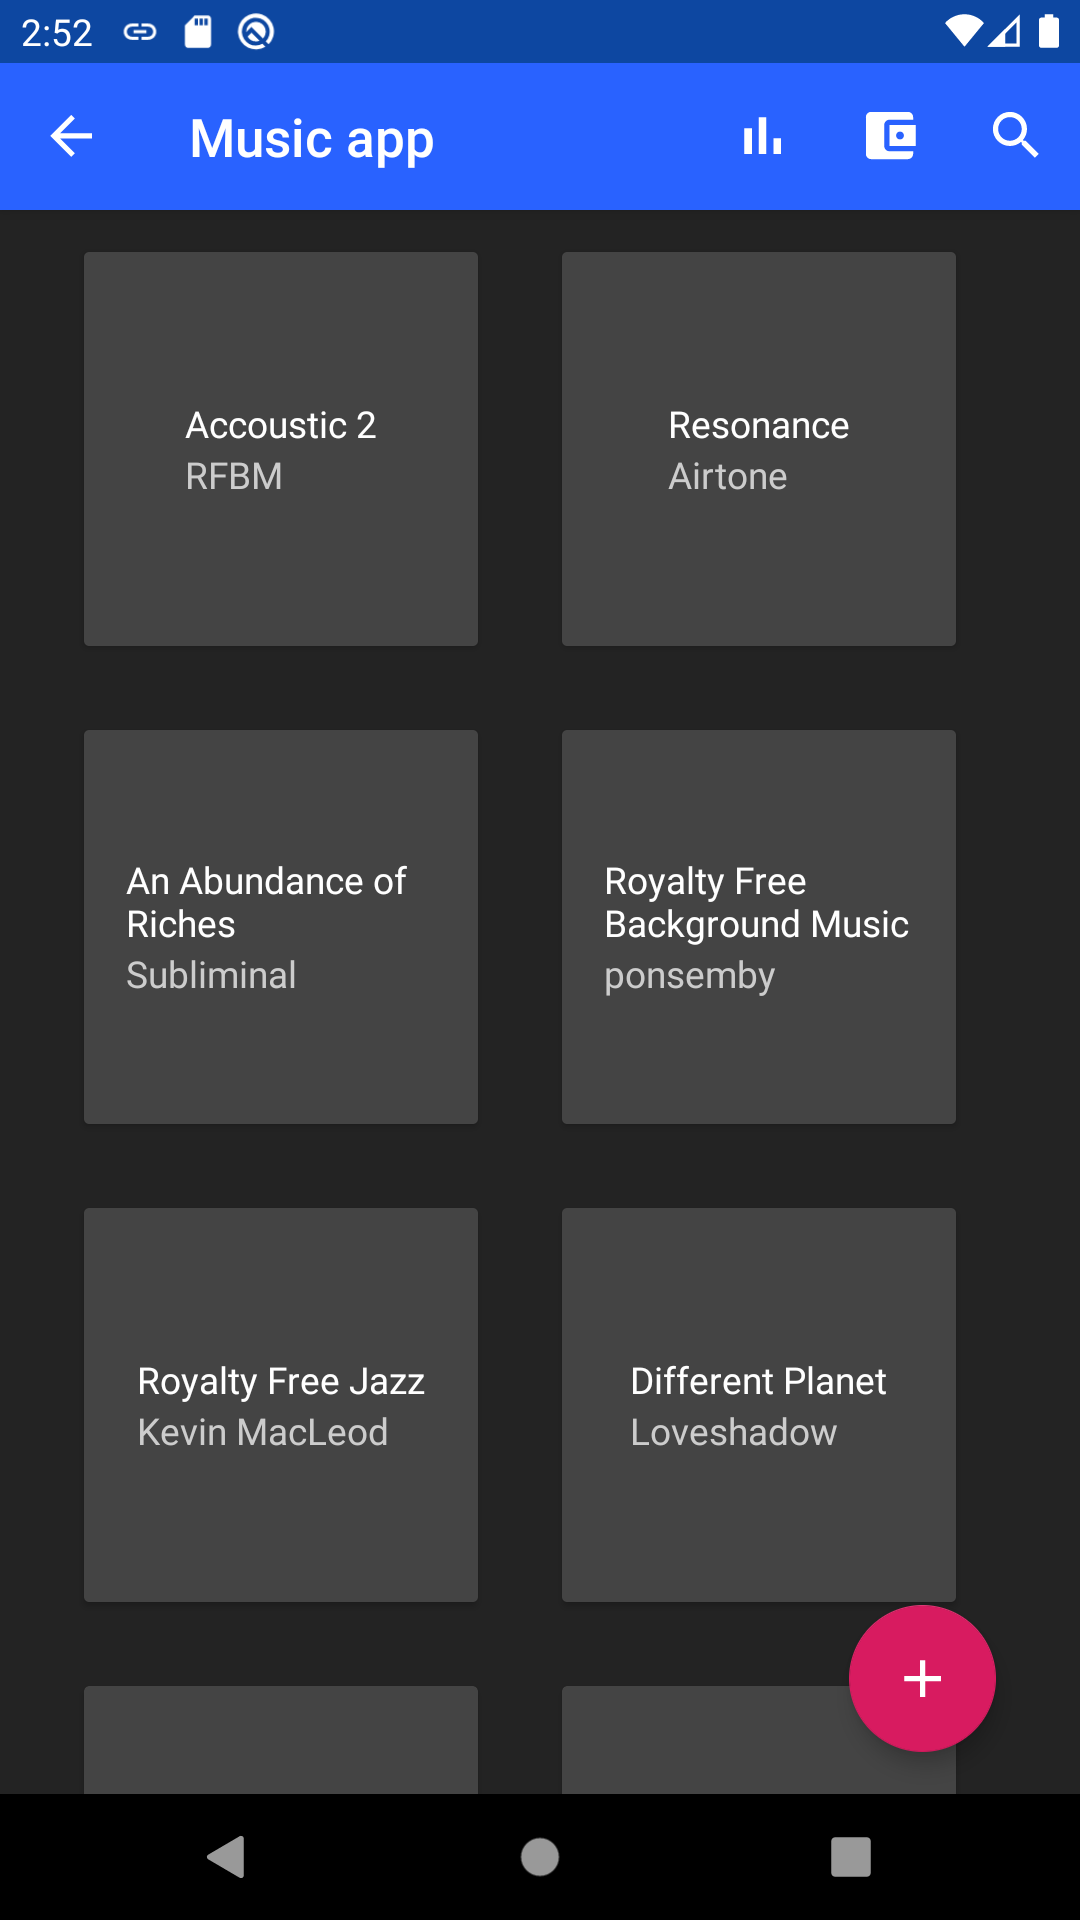
\includegraphics[width=1\linewidth]{implementation/screenshot-home.png}
        \caption{The playlist overview screen, which is the entrance screen}
        \label{fig:screenshot-home}
    \endminipage\hfill
    \minipage{0.3\textwidth}
        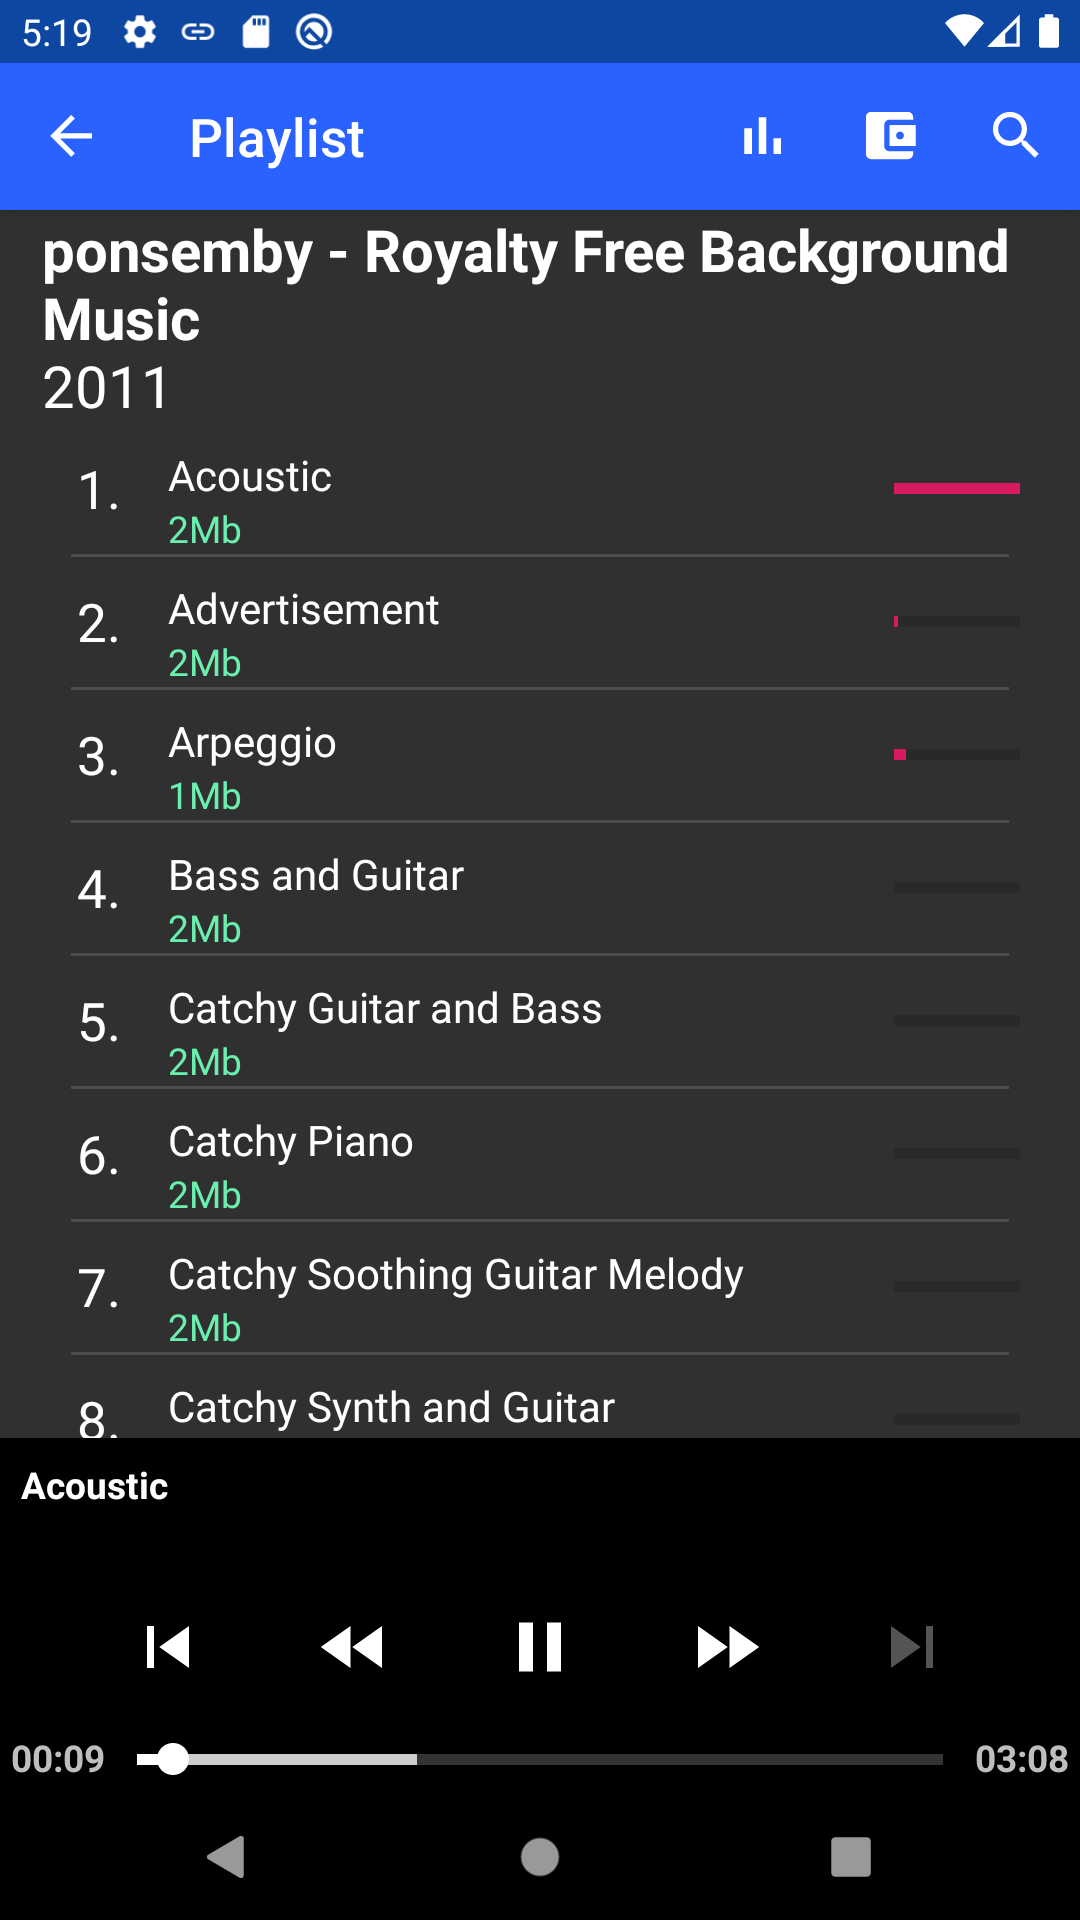
\includegraphics[width=1\linewidth]{implementation/screenshot-playlist.png}
        \caption{Playlist fragment, showing all tracks of one Release}
        \label{fig:screenshot-playlist}
    \endminipage\hfill
    \minipage{0.3\textwidth}
        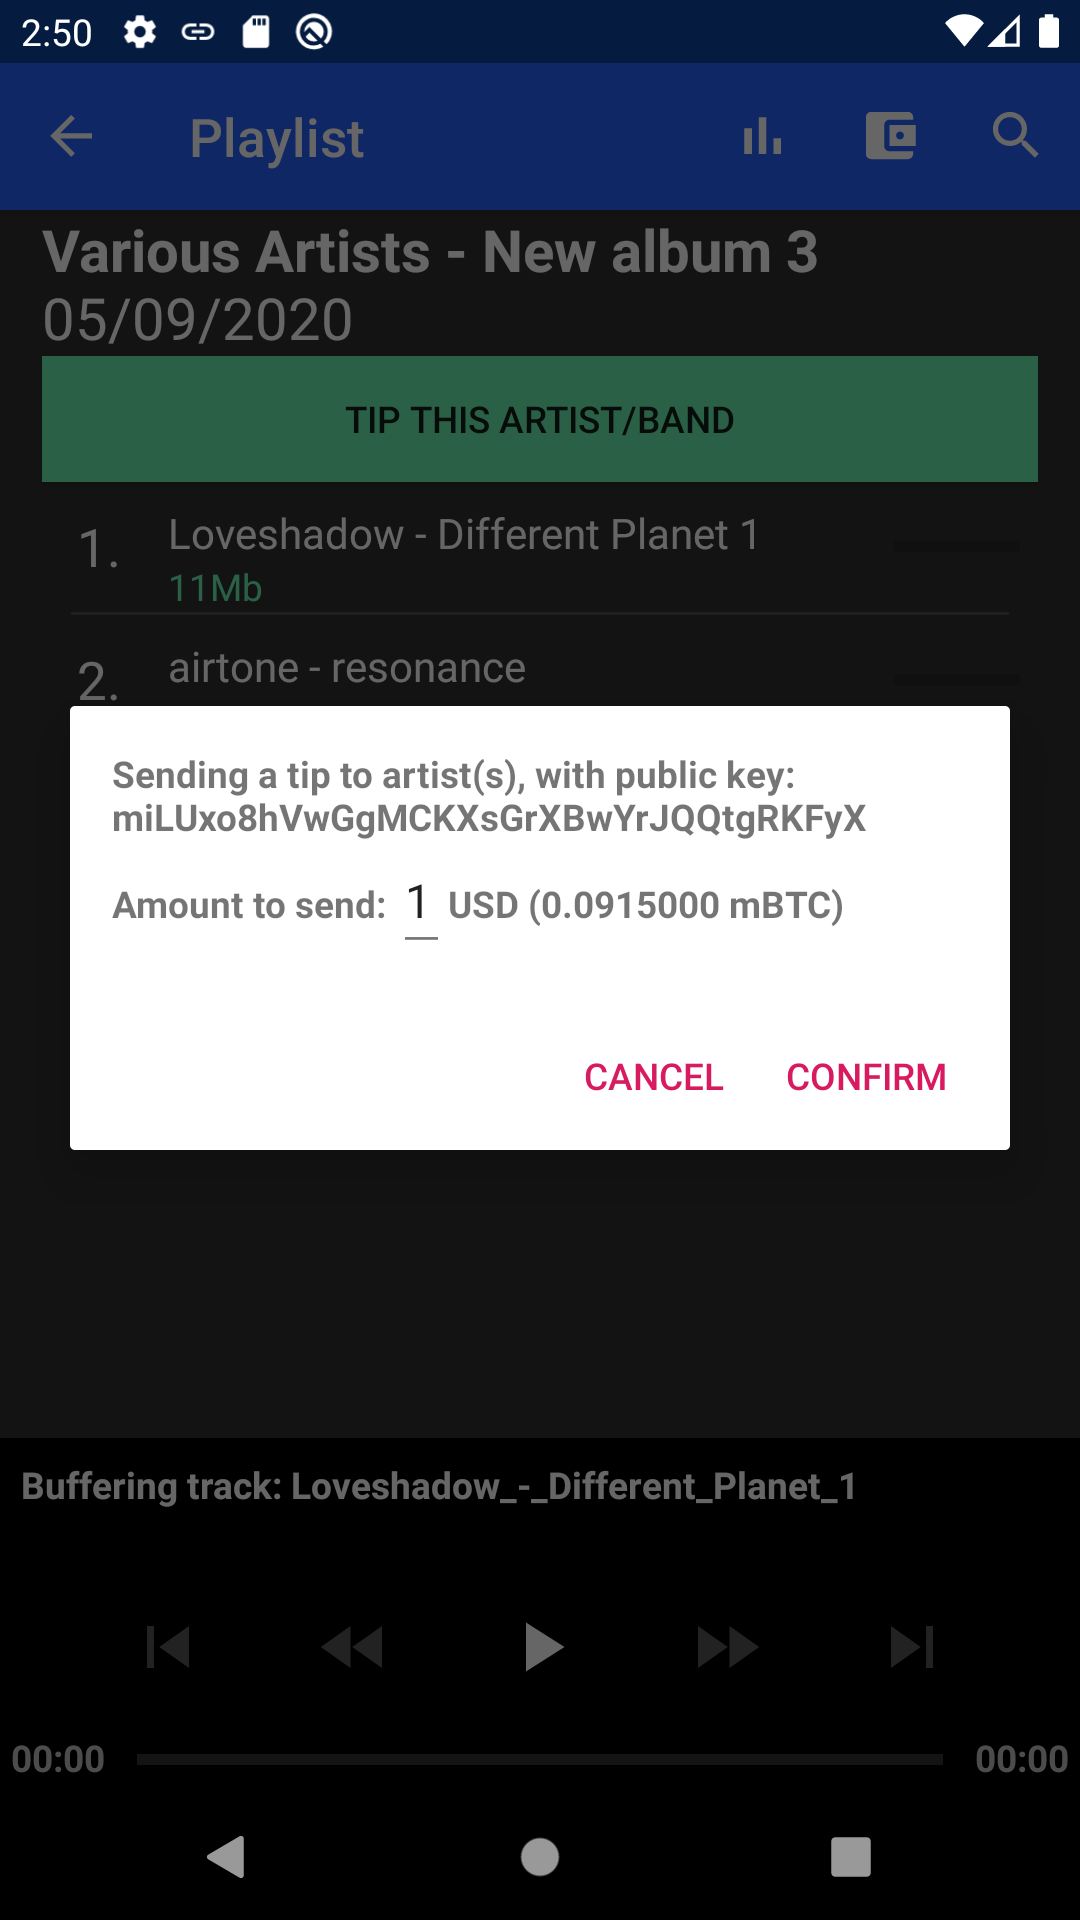
\includegraphics[width=1\linewidth]{implementation/tip-artist.png}
        \caption{Sending a tip to an artist or band}
        \label{fig:tip-artist}
    \endminipage
    % \minipage{0.3\textwidth}
    %     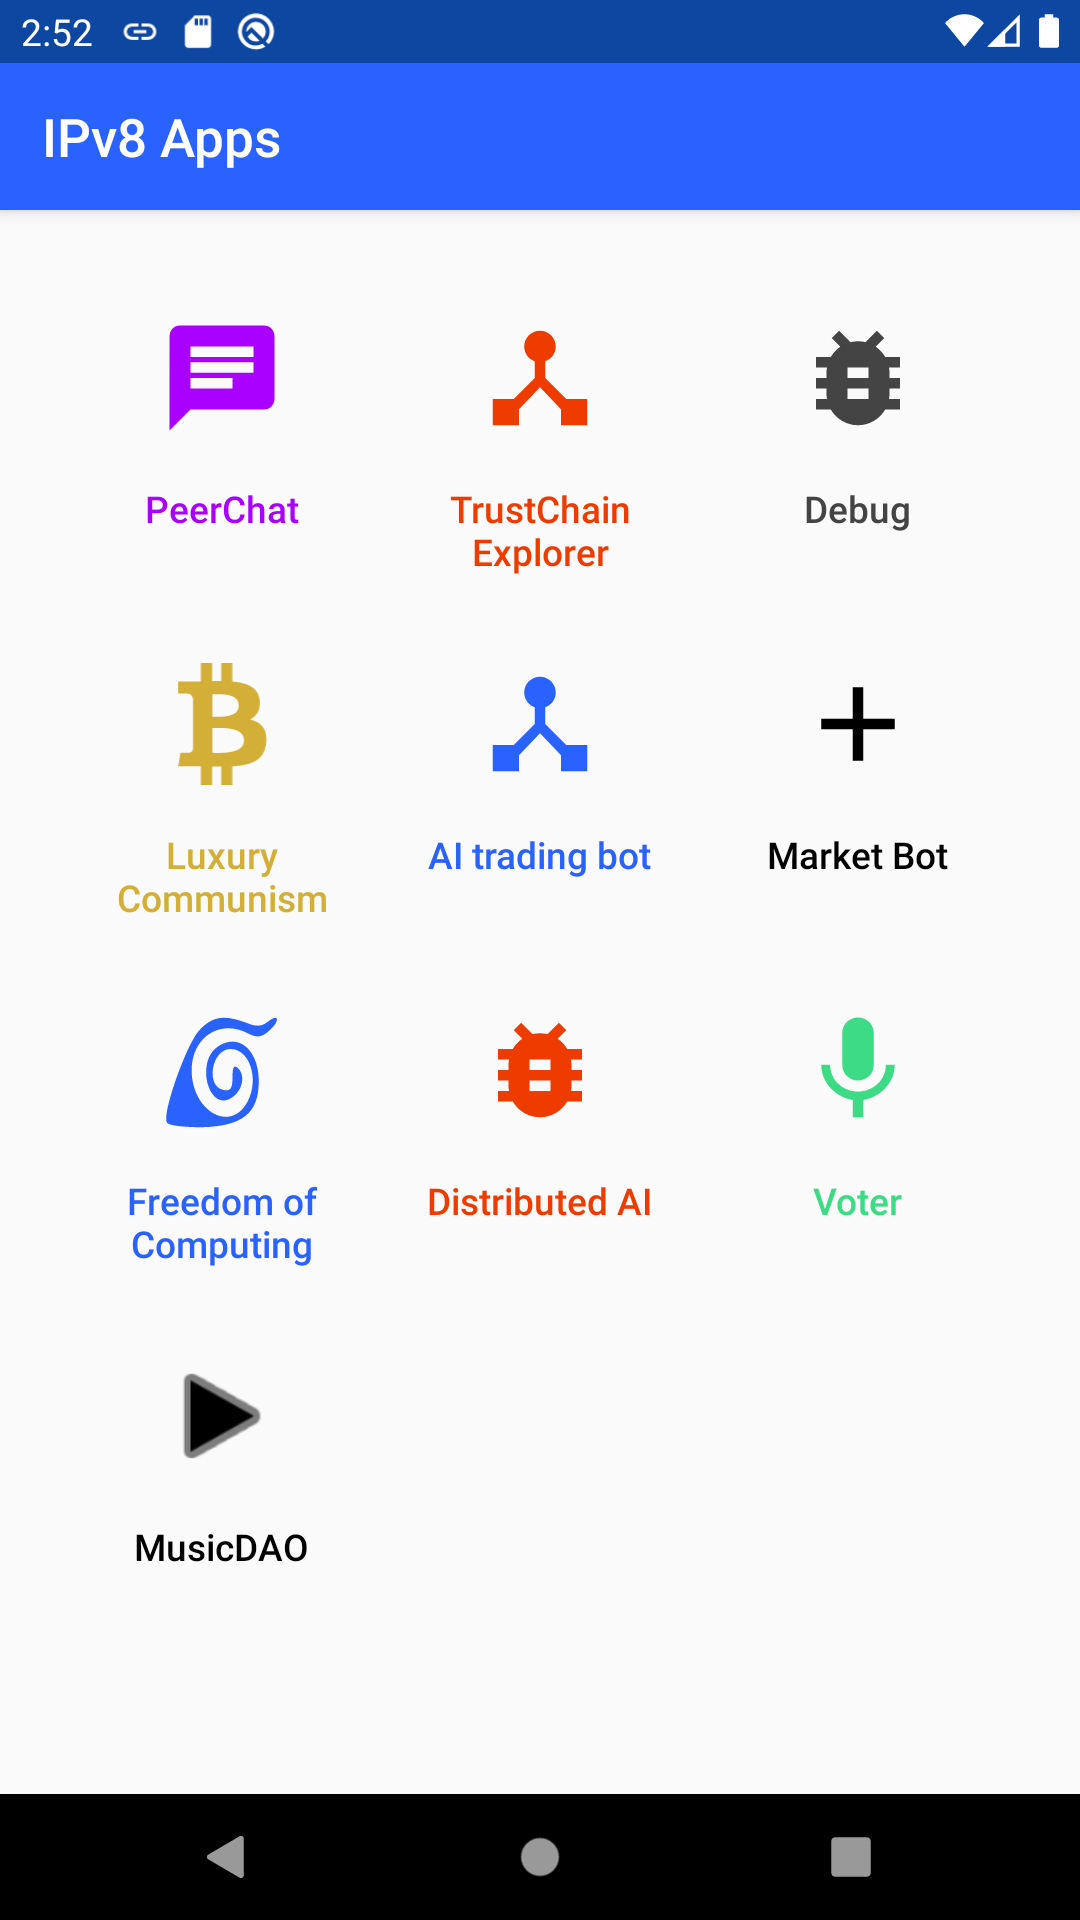
\includegraphics[width=1\linewidth]{implementation/screenshot-superapp.png}
    %     \caption{The app is integrated as a mini-app in the IPv8 Superapp catalog}
    %     \label{fig:screenshot-superapp}
    % \endminipage\hfill
\end{figure}

\section{Playlist overview interface}
The entry point of the app is the playlist overview screen (see \ref{fig:screenshot-home}). It is the screen that is first shown upon starting the MusicDAO. Here the user is presented a list of playlists, with title and author, loaded from local disk and from peers. In our current implementation, each Playlist fragment corresponds to exactly one Release block (see \ref{fig:release-model}). MusicDAO does not support user-made playlists as of the time of writing. The playlists are rendered in real-time based on TrustChain data. This means: during browsing, newly clickable playlists show up instantly once they are discovered from peers. The playlists are sorted on their torrent swarm health in ascending order. Caching is used for fast browsing and music playback. All torrent metadata and all track files received from peers are cached on the Android phone. 
\section{Playlist fragment interface}
When the user selects a playlist to browse and play, this fragment is shown (see \ref{fig:screenshot-playlist}). Here, the user can select a track to play. It presents its list of tracks and other metadata, such as the title and artist(s). For each track the file size is displayed, and a loading indicator on the right side. This shows, in real time, how much of the track is downloaded. In the example of \ref{fig:screenshot-playlist}, the first track is fully loaded. The track player, shown on the bottom, interacts directly with the tracklist and the selected track. It shows which track is selected and whether it is currently playing or buffering.
\section{Wallet interface}
Each device participating in the MusicCommunity is given a private/public wallet identity upon installation of the MusicDAO. The wallet interface (fig. \ref{fig:wallet-sync}) shows synchronization status of the RegTest network (see \ref{sec:regtest-network-impl}). Once the wallet is fully synchronized with the blockchain, the private key and balance are displayed as shown in fig. \ref{fig:wallet-balance}. 

Upon browsing a playlist, a donation button is displayed as shown in fig. \ref{fig:tip-artist}. When pressing this button, the user can select an amount and make a direct donation to the artist or band, in the form of a bitcoin transaction from their wallet. The user enters a value in USD and the corresponding amount in bitcoin is calculated and shown when this field is edited. This is implemented using an external trading platform API\footnote{\url{https://github.com/knowm/XChange/releases/tag/xchange-5.0.1}}\footnote{\url{https://www.binance.com/en/trade/BTC_USDT}}. After confirmation, the transaction is registered on the RegTest network (see \ref{sec:regtest-network-impl}). 

Side note: querying a trading platform API for currency rates makes the app reliant on an external server to run, which is not the aim of this thesis. However this function can trivially be removed without further implications on the system. The current system contains the function to improve the user experience.
\begin{figure}
    \minipage{0.3\textwidth}
        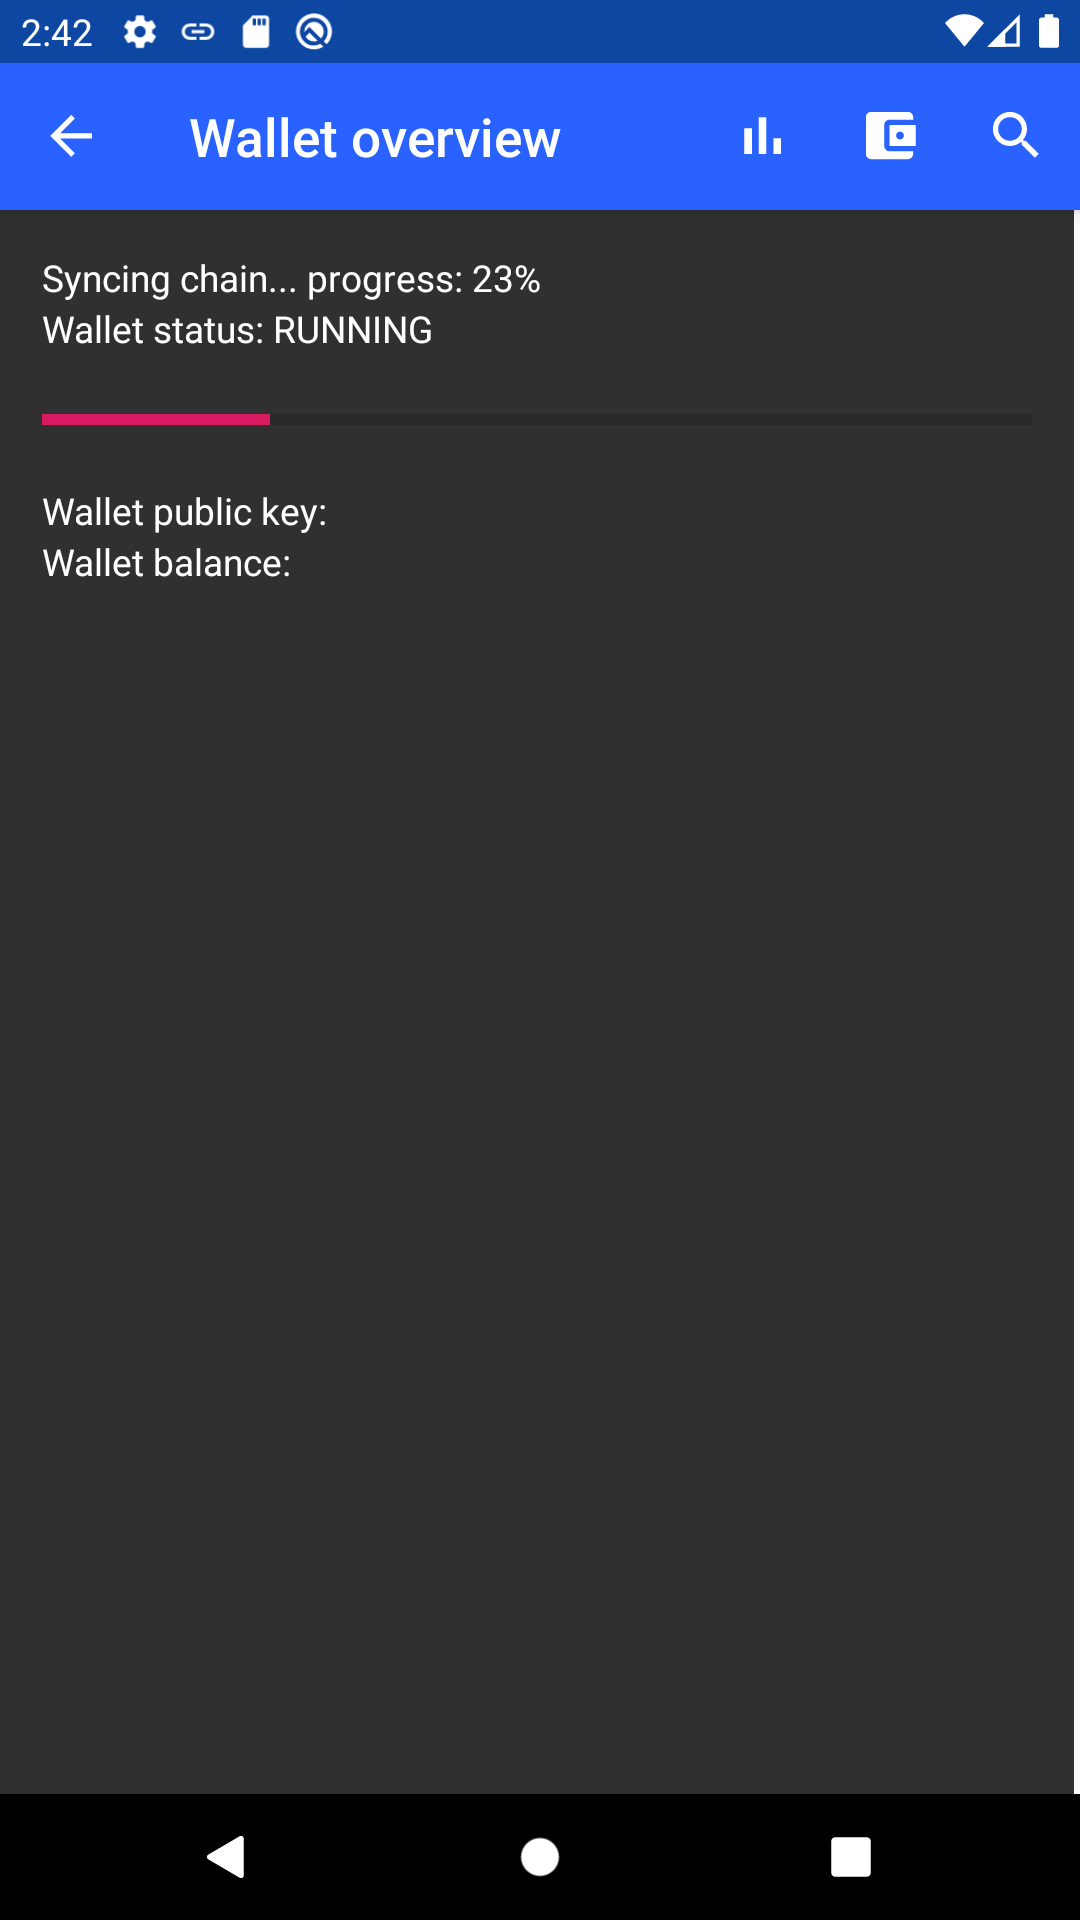
\includegraphics[width=1\linewidth]{implementation/wallet-sync.png}
        \caption{Synchronizing with the Bitcoin RegTest environment blockchain}
        \label{fig:wallet-sync}
    \endminipage\hfill
    \minipage{0.3\textwidth}
        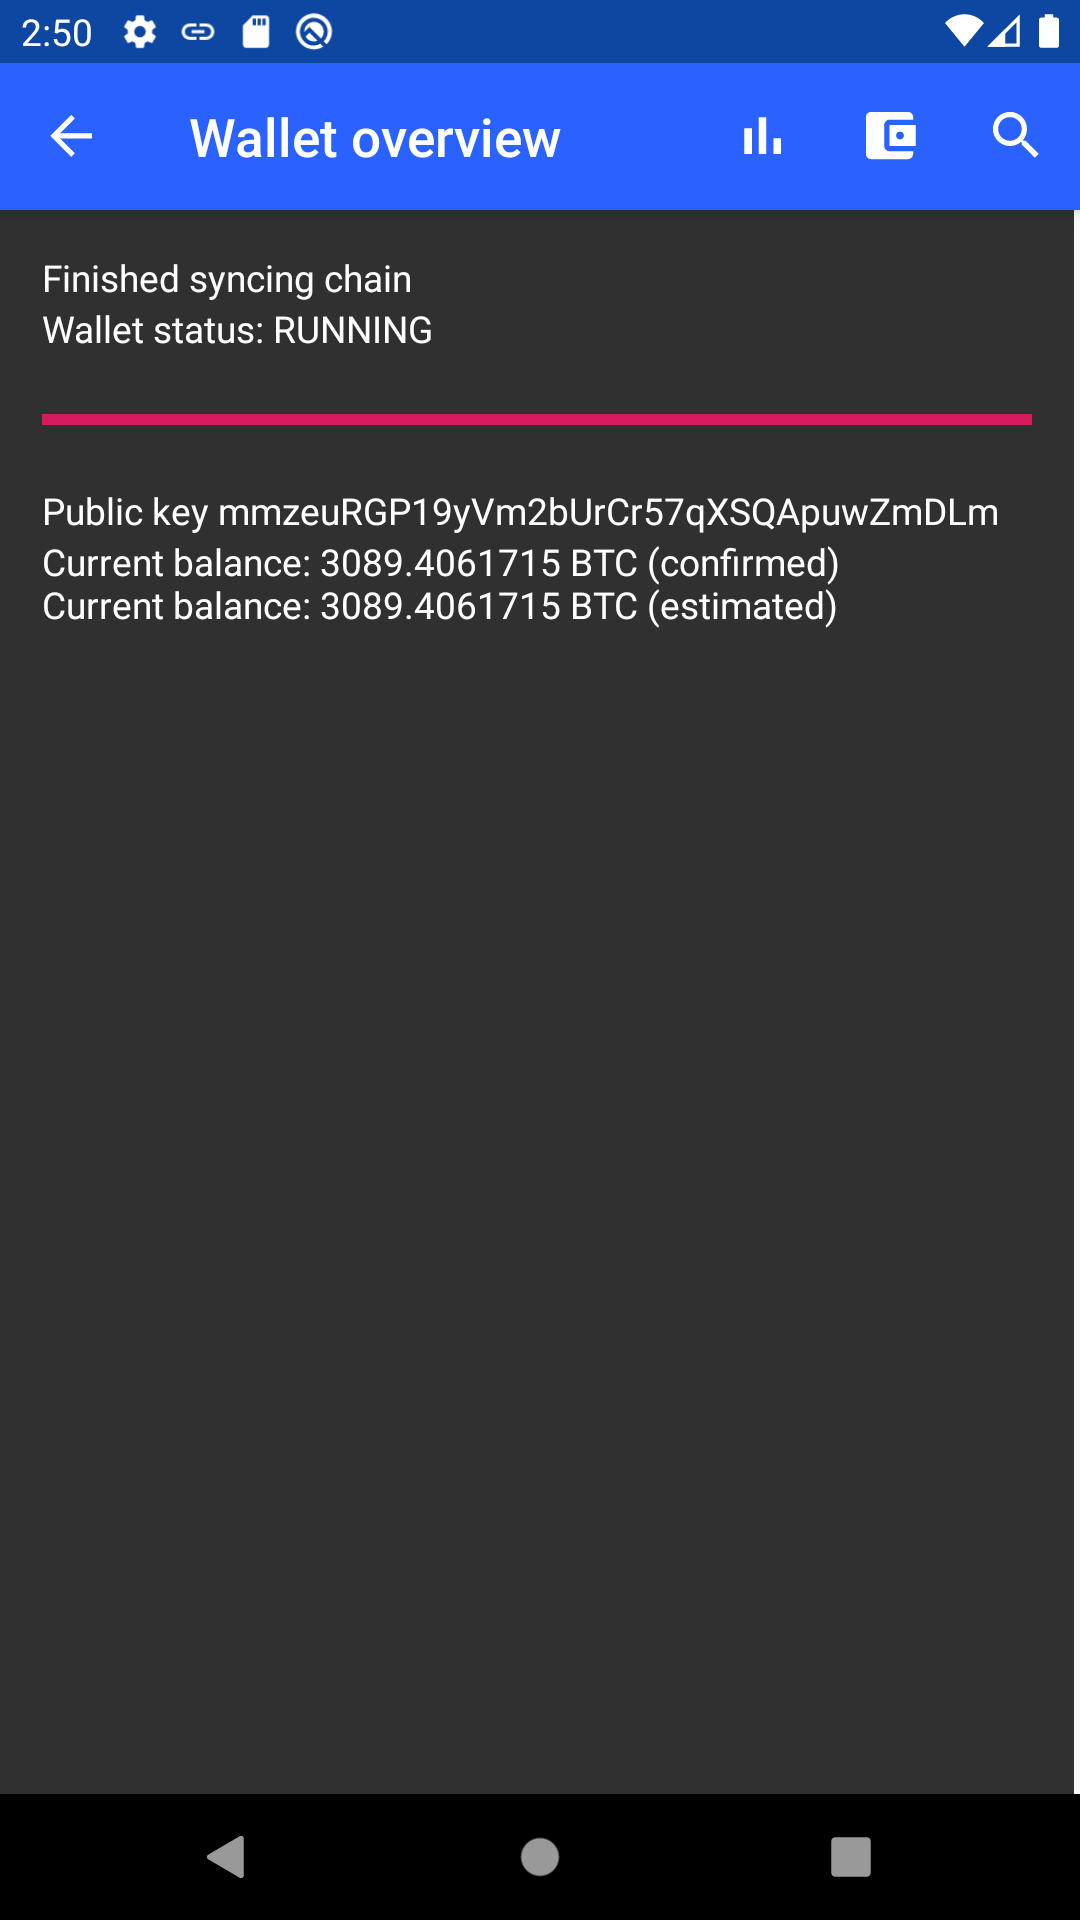
\includegraphics[width=1\linewidth]{implementation/wallet-balance.png}
        \caption{Wallet overview and balance after synchronizing}
        \label{fig:wallet-balance}
    \endminipage\hfill
    \minipage{0.3\textwidth}
        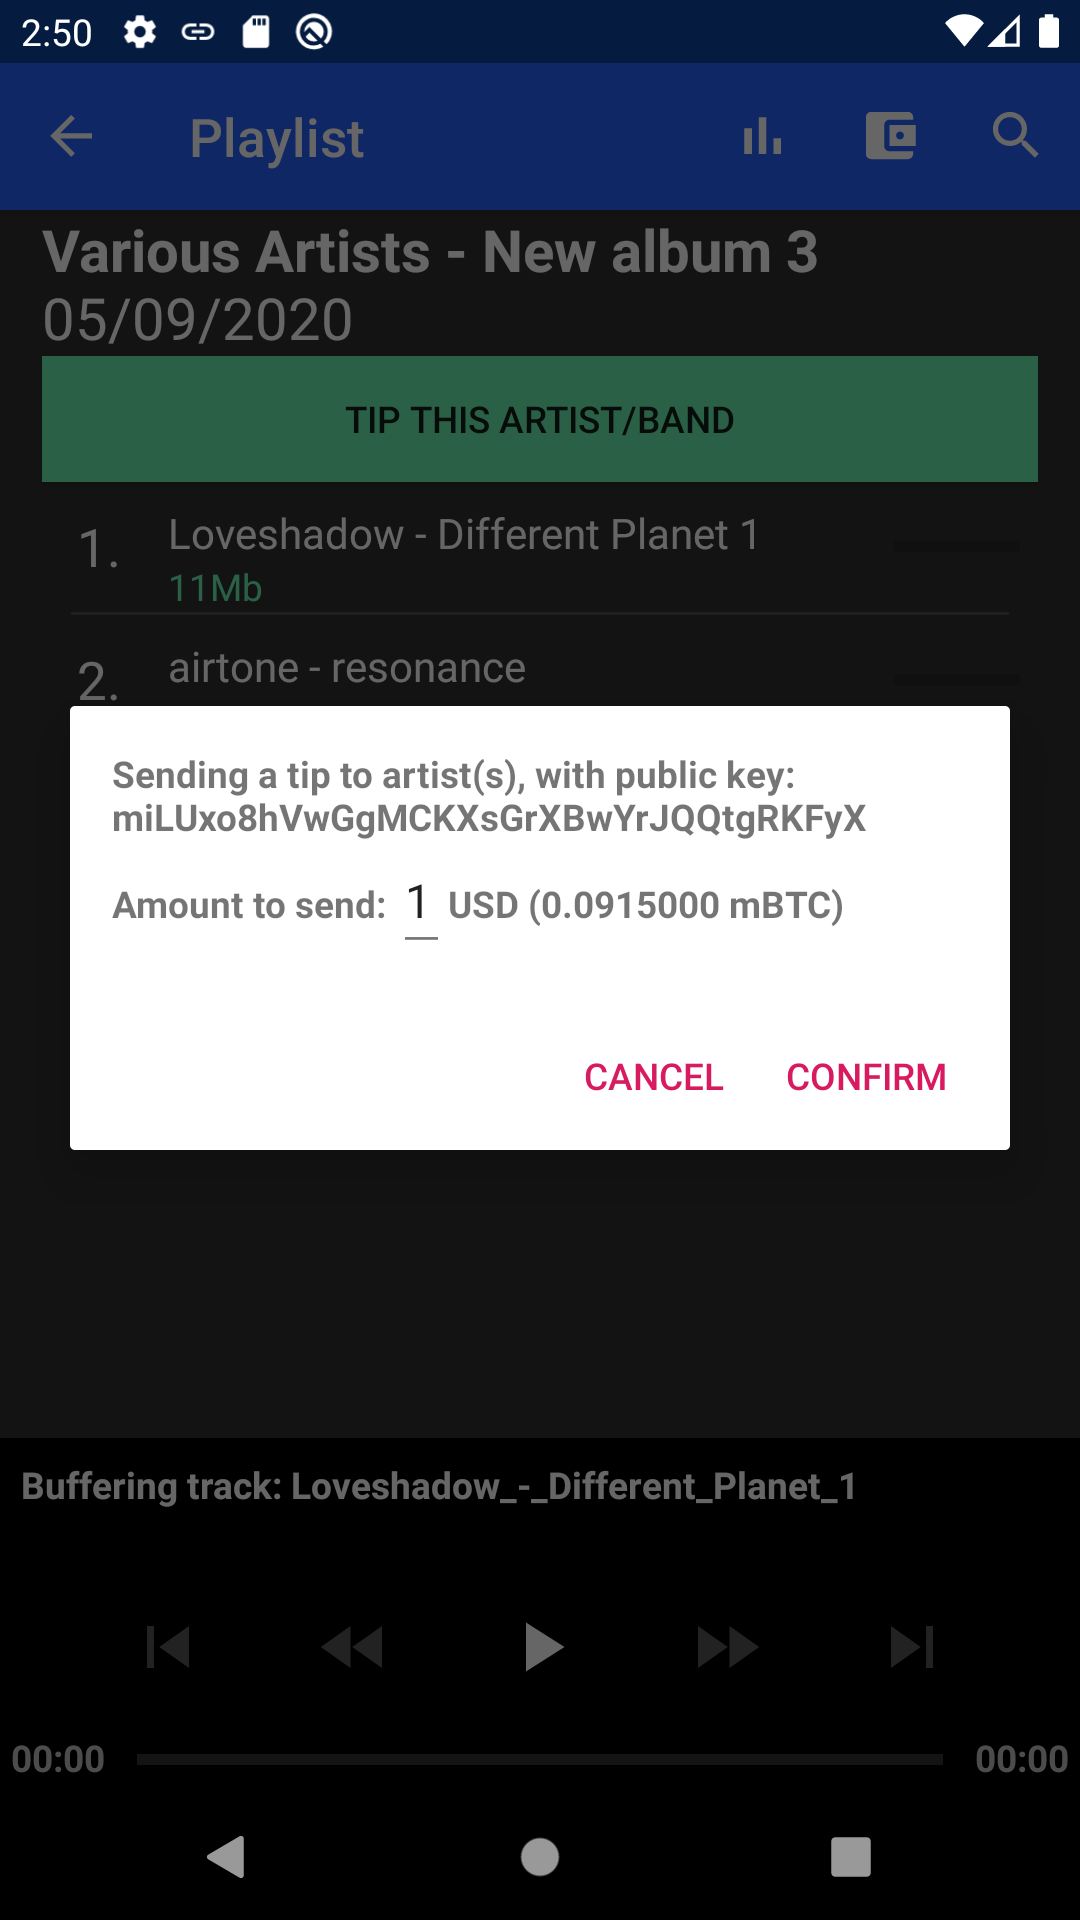
\includegraphics[width=1\linewidth]{implementation/tip-artist.png}
        \caption{Sending a tip to an artist or band}
        \label{fig:tip-artist}
    \endminipage\hfill
\end{figure}

\section{Networking}
We implement audio track uploading, downloading and streaming using JLibtorrent\footnote{\url{https://github.com/frostwire/frostwire-jlibtorrent}}, an implementation of BitTorrent. Immutable and public storage of metadata is implemented with TrustChain~\citep{otte2017trustchain}. 
% This technology has shown to run well on mobile devices (cite), and allows for extensive configuration.
\subsection{Release creation and sharing}
\label{sec:torrent-creation}
To create and share music content, a user can create a Release object using the dialog shown in fig. \ref{fig:submit-release-dialog}.  There are two options for creation: the user either selects local audio tracks or pastes a magnet link. Afterwards, the user adds metadata describing the contents and submits the Release. In the background this creates a torrent file, which is stored on the mobile device. Finally, by using the computed infohash and file list, the magnet link of the torrent file is created and added to the \textit{magnet} field of the Release block.

We use trackerless torrents, to keep the network decentralized. Instead of relying on centralized trackers, peers are found using a distributed hash table~\citep{dht2019}. In addition, the app uses the local peer discovery (LPD)~\citep{bittorrentbep142015} functionality of BitTorrent. This allows for finding peers and transmitting torrent pieces over a LAN, resulting in fast transmission and low latency.
\subsection{Content seeding}
\label{sec:content-seeding}
Seeding of content is implemented using a simple continuous mechanism. The ContentSeeder class runs a background thread which seeds all local torrents, with an upper threshold \(T\). This is set to \(T=10\). The ContentSeeder uses a last-in-first-out heuristic: Only the top \(T\) most recently created/received torrent files are seeded.

\begin{figure}
    \minipage{0.3\textwidth}
        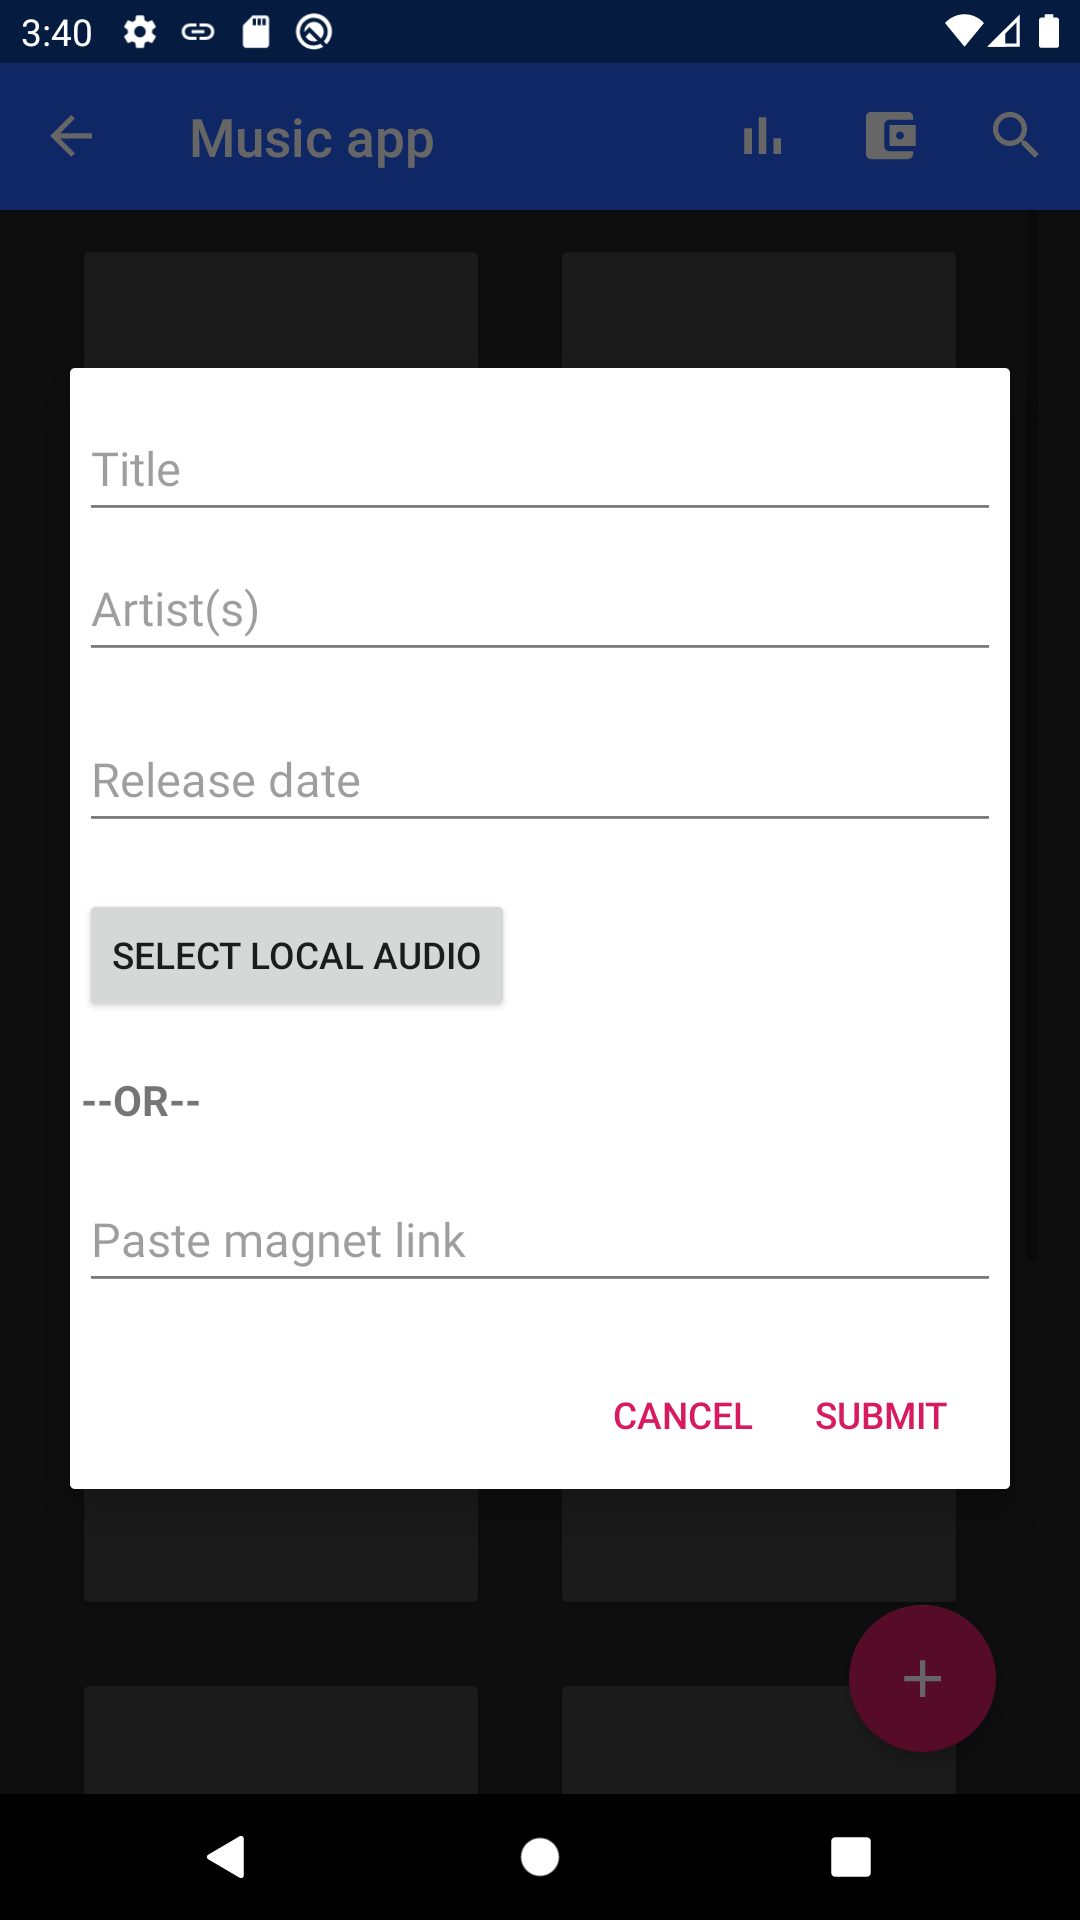
\includegraphics[width=\linewidth]{implementation/screenshot-select-tracks.png}
        \caption{Dialog for creating and publishing a new Release}
        \label{fig:submit-release-dialog}
    \endminipage\hfill
    \minipage{0.6\textwidth}
    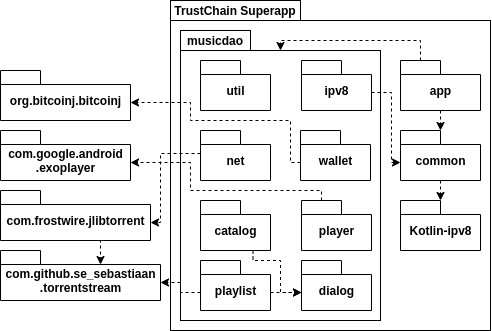
\includegraphics[width=1\linewidth]{implementation/package-diagram.png}
        \caption{Package diagram showing the interaction with external libraries and TrustChain Superapp packages}
    \label{fig:package-diagram}
    \endminipage
\end{figure}

\section{Music Player and Streaming} 
Playing music is implemented using ExoPlayer (\ref{tab:library-usage}). This music player library is suitable as it allows for playing tracks that are partially loaded, which enables streaming.
\subsection{Priority handling}
To achieve fast buffering, we implemented a priority system for tracks and for parts of tracks (chunks). In essence, the player prioritizes chunks that the user is currently interested in, by actively asking peers to send the corresponding chunks that are necessary to play the selected section of the track. In addition, the selected track is given a higher priority over other tracks in the playlist.

This uses the piece priorities system in libtorrent, which range from 1 (normal) to 7 (highest) (see libtorrent Manual\footnote{\url{https://www.libtorrent.org/manual-ref.html\#file-format}}). By default, the first couple of chunks of each track are given a high priority, to reduce the chance of buffer underflow, so that the user can start streaming early.

\section{Identity and authenticity}
Every device participating in MusicDAO has a unique identity. MusicDAO implements the public-key infrastructure as described in \ref{sec:pki-design} using the identity system proposed by \cite{mattskala2020}. This uses the \textit{Curve25519} cryptography system. Using this system, it is computationally infeasible to obtain the private key from a  public key. For simplicity in implementation, we assume that every device in the network is an abstraction of a unique artist. 

All immutable music release blocks are assigned an identity of the creator using a public key. Every device running the MusicDAO will receive a public/private key-pair upon first launch. 

Currently there is no multi-signature support implemented. This means that in the case of a group publishing a Release, there is only one public key representing the whole group. Every artist, and every unique collaboration between artists should generate their own key-pair to describe ownership of the Release.
%  This is a public key using \textit{Curve25519} elliptic-curve cryptography. 

% \section{Metadata storage and discovery}
% \subsection{Release blocks}
% Releases are objects that represent an audio release produced by one or more artists. This can be an album, an EP, a single, or a podcast. Release objects are stored on the TrustChain, and are exchanged between peers that are part of the MusicCommunity (see \ref{sec:searching-musiccommunity-impl}). These objects are structured as shown in \ref{fig:release-model}. The \textit{magnet} property contains a magnet link which holds all additional information about the contents of the Release, such as the torrent file list, size and tracker URLs. The \textit{publisher} property contains the public key of a Bitcoin wallet which is owned by the creator of the Release. This public key is an identity of the owner of the record (either the artist, band or label). This allows only the owner to receive funds sent by listeners, and no other middlemen (apart from miners).
% % When a torrent is created from a local file list, the TorrentInfoName value is established. 

\subsection{Keyword search}
\label{sec:searching-musiccommunity-impl}
The app allows users to search for music content remotely using keyword search. The search function tries to find matches locally, and if there are only a few found, it will try to ask for content from peers. We implemented algorithm 1 for this functionality. The current implementation uses only a simple filter, which checks if the keyword is contained in the metadata of the music release.

When the user performs a search, the local database is filtered first to find matches. If there are unsatisfactory results, it sends a \textit{KeywordSearchMessage} (see \ref{fig:keyword-search-message-model}) to a few random peers. This asks neighbours to inspect their local database to find matches for the same query. If the peer finds a match, it sends the corresponding results directly back to the original asker. To disallow packages from endlessly being forwarded on the network we use a time-to-live property. For details, refer to algorithm 1.

\section{Donations and payments}
\label{sec:regtest-network-impl}
Our system contains peer-to-peer payments where 100\% of money goes to artists. We created a public Bitcoin RegTest environment\footnote{\url{https://developer.bitcoin.org/examples/testing.html\#regtest-mode}} to test peer-to-peer Bitcoin donations and payments. This creates a new `clean slate' Bitcoin blockchain and allows for full control over the chain and miners. This enables a test environment that is useful for experiments, as we can tweak the block generation speed and keep track of all transactions registered on the blockchain. 

Each device must be synchronized with the network in order to make payments. A background thread of MusicDAO establishes and maintains communication with bitcoin nodes, so that it does not interrupt the user experience. The progression of synchronization can be seen in the wallet interface. Synchronization with the RegTest network is done using a single bootstrap server, which is a hard-coded address in the app. This is necessary for running on a test net, as it will take an infeasible amount of time to guess the address of a running Bitcoin node, with only a few nodes. but in a real-world situation, bitcoin nodes should be found by querying peers for bitcoin node addresses.

In the current system, when a user makes a donation, this donation can only go to one artist. An automatic splitting system between different artists of one group or band has not been implemented yet.

\section{Quality assurance}
In order to preserve quality of code we make use of continuous integration, automated tests and an online crash reporter. Unit tests are written using JUnit 4\footnote{\url{https://junit.org/junit4/}} and the mocking library Mockk\footnote{\url{https://mockk.io/}}. The code coverage of these unit tests can be seen in \ref{tab:code-cov}. 

Code coverage is measured by Android Studio 4\footnote{\url{https://developer.android.com/studio}}. The majority of uncovered code contain user interface interaction and networking callback logic. Code coverage could have been improved by introducing Android instrumented tests. These are tests that run on an Android device or emulator so that user interaction flows can be tested. However, we chose to not implement this as these type of tests can not be run in our continuous integration environment, and tweaking the CI for support of this would be a non-trivial task.

All tests are run in an automated testing environment using Github Actions\footnote{\url{https://github.com/features/actions}}. This continuous integration system is executed on every pull request for changes to the code. Aside from this, during the experimentation phase, app installs and crashes are recorded using Firebase Crashlytics, which is an end-to-end crash reporting tool. It shows details of each application crash of all users (see fig. \ref{fig:firebase-crashlytics}). Using this, a full stack trace can be inspected remotely for each crash. In addition it helps with gaining insight in performance for certain types of Android devices, Android versions and helps us evaluate user interaction with the app.

\begin{table}[]
\begin{tabular}{|l|l|}
\hline
\textbf{Package/class} & \textbf{Line coverage} \\ \hline
MusicService.kt        & 15\% (15/95)           \\ \hline
MusicBaseFragment.kt   & 50\% (1/2)             \\ \hline
catalog                & 24\% (35/142)          \\ \hline
dialog                 & 20\% (24/130)          \\ \hline
ipv8                   & 81\% (57/70)           \\ \hline
net                    & 90\% (27/30)           \\ \hline
player                 & 0\% (0/50)             \\ \hline
playlist               & 9\% (19/203)           \\ \hline
util                   & 60\% (42/70)           \\ \hline
wallet                 & 0\% (0/100)            \\ \hline
\end{tabular}
\caption{Code coverage overview}
\label{tab:code-cov}
\end{table}

\begin{figure}
    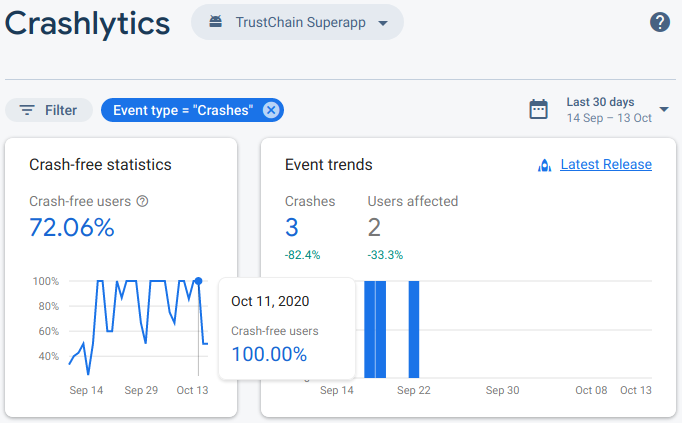
\includegraphics[width=0.8\linewidth]{implementation/firebase-crashlytics.png}
    \caption{Firebase Crashlytics crash reporter; this figure shows the crashes over time}
    \label{fig:firebase-crashlytics}
\end{figure}